\section{Motivation}
	In this section, we use a classical control example to explain the motivation behind this work. Consider the problem of designing stablizing control for an inverted pendulum which takes (polytopic) constraints over state variables and control inputs into account. The linearized continuous-time description for the open-loop system's dynamics is as follows:
	\begin{equation}
		\begin{bmatrix}
			\dot \theta\\
			\dot \omega
		\end{bmatrix}=
		\begin{bmatrix}
			0 & 1\\
			\frac{g}{l}& \frac{-b}{ml^2}		
		\end{bmatrix}
		\begin{bmatrix}
			\theta\\
			\omega
		\end{bmatrix}+
		\begin{bmatrix}
			0\\
			\frac{1}{ml^2}
		\end{bmatrix}u
		\label{eq:pendul_ss}
	\end{equation}
	where, $\theta$, $\omega$ and $u$ denote angular position, angular speed and input torque respectively; $g=9.81 m/s^2$ is the gravitional acceleration, $m$ the ball mass, $b$ the rotational fraction coefficient and $L$ the length of the bar. To design the controller, one has to first descretize the dynamics in $\eqref{eq:pendul_ss}$ with respect to an appropriate sample time $T_s$. Starting from an initial state, we would like the system's trajectory to converge into its equilibrium point while always $\theta\in[-\pi,\pi]$ and $\omega\in[-\pi/8,\pi/8]$. While there are many control schemes which can be used to stablize the system (e.g. LQR, state feedback), adding polytopic constraints, MPC schemes will be the best choice. 
	%In literature, many control schemes are proposed for stablizing the system around the equilibrium point. 
	%In order to design a controller which takes additional safety constraints are taken into account, model predictive control (MPC) schemes seem to be best candidate. 
	However, one major challenge for implementing model predictive controllers over embedded systems will be to solve MPC optimality problem within each time step. Since the system under consideration is LTI, one can use explicit MPC scheme proposed in [Bemporad:2002] which computes partitions over state space together with affine functions which computes the optimal control input over their corresponding partition. For the inverted-pedulum example, the computed optimal control contains $14$ partitions shown in Fig \ref{fig:pendulum_reg}.
	%To overcome this issue, in [Bemporad:2002], explicite MPC, a multi-parametric programming based approach is proposed for LTI systems. 
	In practice, EMPC will be implemented over relatively low-price embedded systems which have limited memory capacity and computational power. Computing the optimal control input can be efficiently done using for example binary tree search. However, the memory limit is more serious as it increases proportional to the number of partitions.	Therefore, one direction is to explore ways to reduce required memory.
	On the other hand, most of the industrial embedded systems over which EMPC is implemented, only support fixed point arithmetic. Using fixed point arithmetic, will cause approximation error that is inversely proportional to the number of bits used. This approximation error must be considered since it might lead into violation of problem constraints. Therefore, one need to formulate the problem as robust MPC to count for disturbance input $|\omega|\leq \bar\omega$. Setting the number of bits for storing different variables, one can compute the upper bound for approximation error, $\bar\omega$. However, we would like to achieve the minimum number of bits that reduces memory requirements. To that end, one approach is to start with an initial $\bar \omega$; design an explicit robust MPC controller with respect to $\bar \omega$ and to use state of the art fixed-point error analyzers to decide for the number of required bits for saving each parameter. Again, back to inverted pendulum example, choosing $\bar \omega=0.1$, we design a robust MPC controller with partitions given in Fig. \ref{fig:pendulum_reg} (b). Now, in order to decide for the smallest number of bits, we use the floating point analysing tool, Daisy, to provide us with minimal uniform and mixed fixed-point reperesentation. 
	
%	\begin{figure}
%		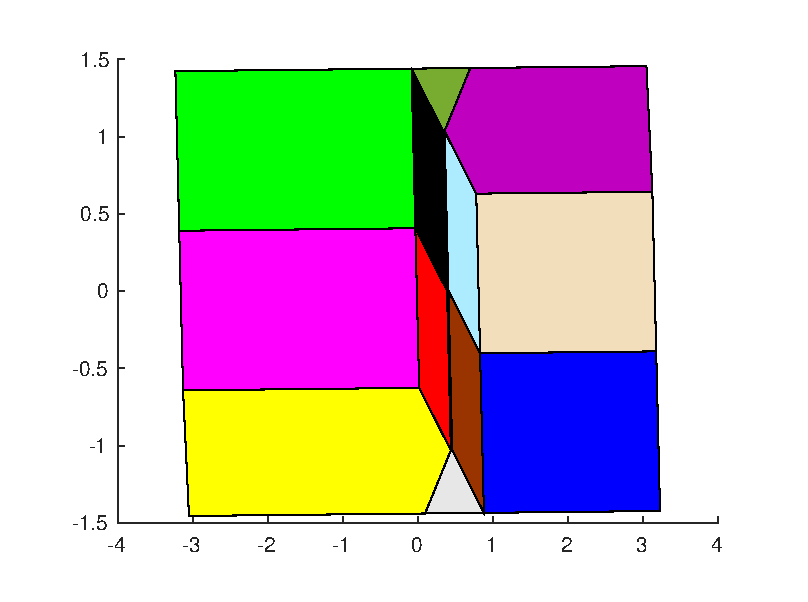
\includegraphics[width=.25\textwidth]{Figs/partition_order2_noise.eps};
%	\end{figure}
	
	
	\tikzstyle{block} = [draw, fill=blue!20, rectangle, 
	minimum height=3em, minimum width=6em]
	\tikzstyle{sum} = [draw, fill=blue!20, circle, node distance=1cm]
	\tikzstyle{input} = [coordinate]
	\tikzstyle{output} = [coordinate]
	\tikzstyle{pinstyle} = [pin edge={to-,thin,black}]
	\begin{figure*}[t]
		\begin{tikzpicture}[auto, node distance=2cm,>=latex',scale=1]
			\centering
			\node [block, pin={[pinstyle]above:$\delta=\delta_0$},
			node distance=5cm] (RMPC) {Robust MPC design};
			%\node[right of=RMPC](partitions){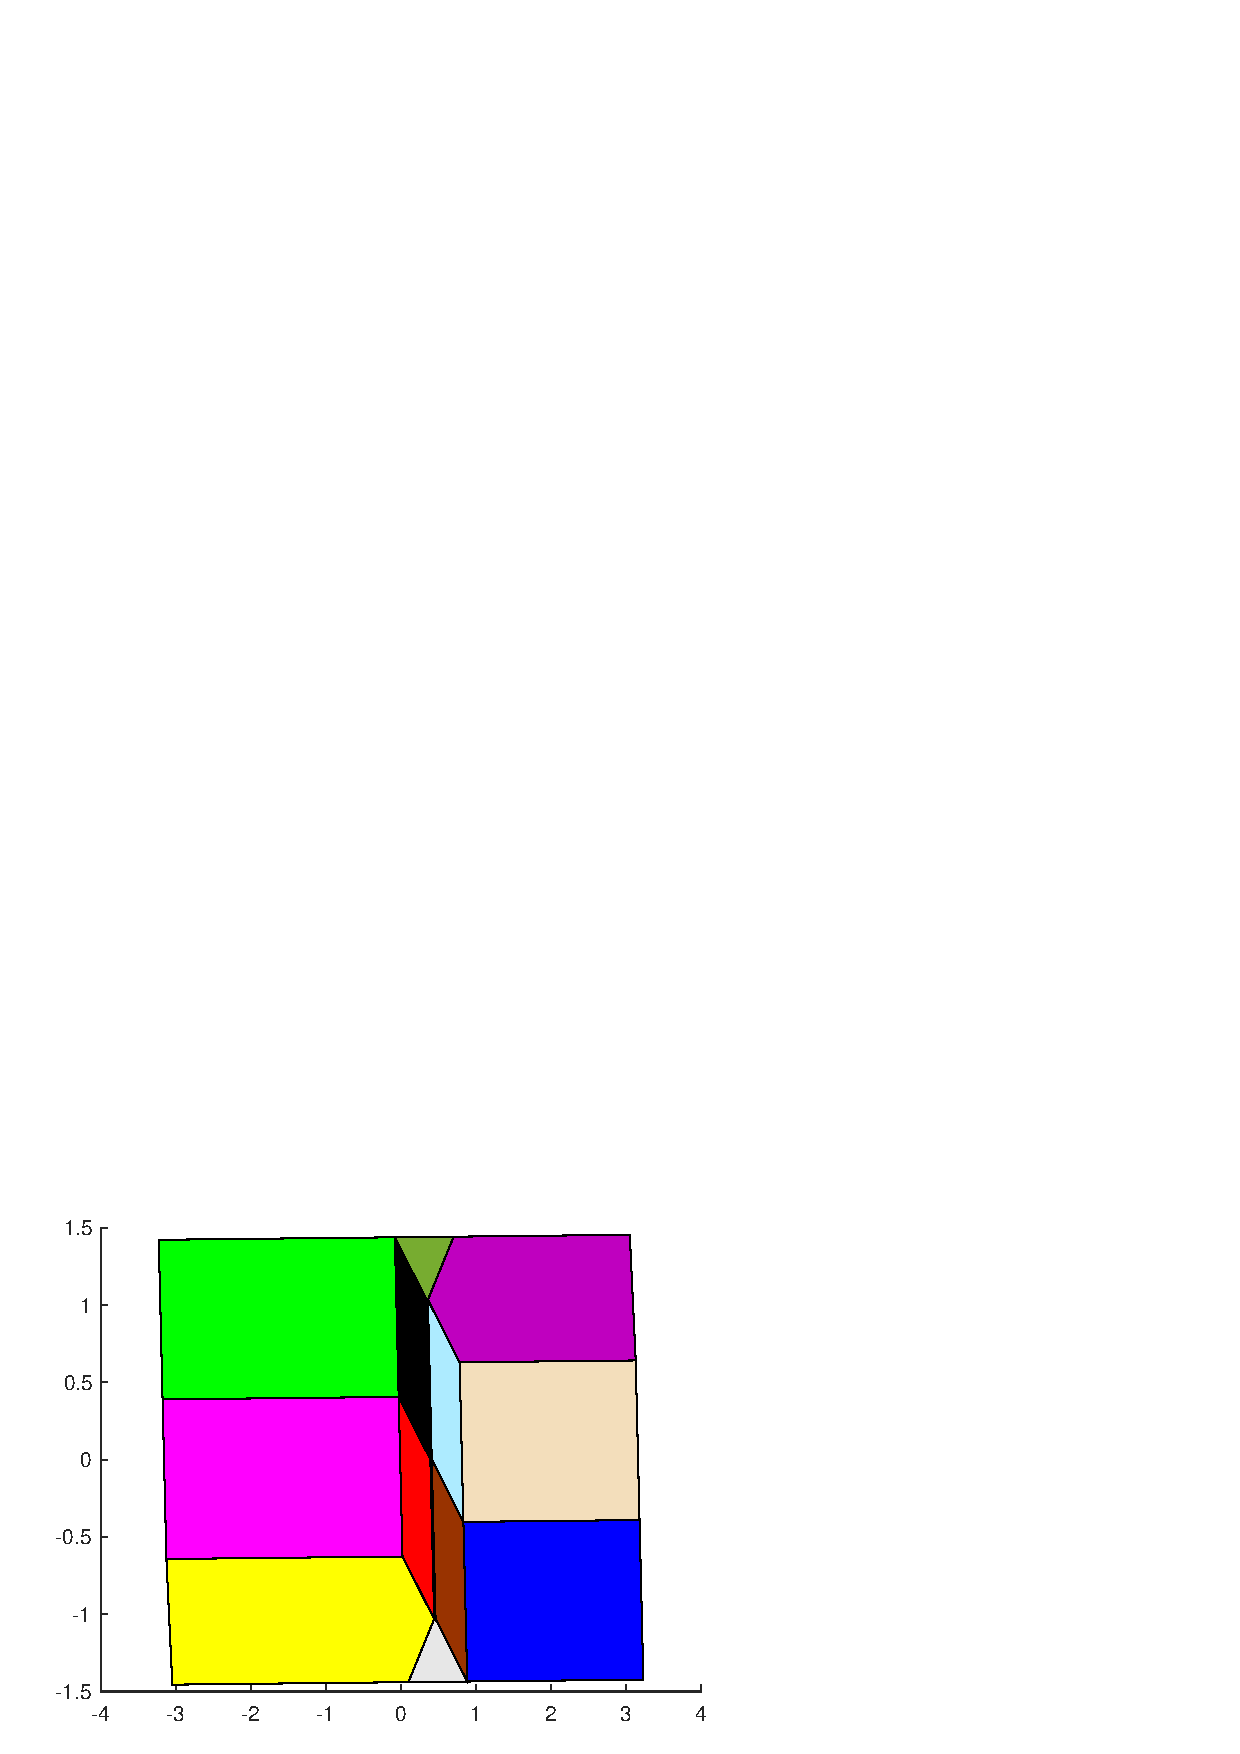
\includegraphics[width=.25\textwidth]{Figs/partition_order2_noise.pdf}};
			\node [block, right of=RMPC,
			node distance=5cm,text width=3cm] (mixed) {Mixed precision analysis};
			\node [draw, fill=blue!20, diamond, 
			minimum height=3em, minimum width=3em, right of=mixed,
			node distance=5cm] (decide) {Is memory violated?};
			\node [block, right of=decide,
			node distance=3cm] (done) {Done};
			\node [block, below of= decide,
			node distance=3cm] (delta) {increase $\delta$};
			
			\draw [draw,->] (RMPC) -- node [pos=-.1] {}(mixed);
			\draw [->] (mixed) -- node [name=aaa] {}(decide);
			\draw [->] (decide) -- node [above,pos=.3] {Yes} (done);
			\draw [->] (decide) -- node[pos=0.99] {} 
			node [] {No} (delta);
			\draw [->] (delta) -| node [above] {$\delta$} (RMPC);
	
	\end{tikzpicture}
	\caption{high level description of RMPC with Daisy}
	\label{fig:overview}
\end{figure*}